\documentclass[logo,reportComp]{thesis}
\usepackage[cpp,linenum]{mypackage}

\title{计算机图形学}
\subtitle{作业六:光照效果}
\school{数据科学与计算机学院}
\author{陈鸿峥}
\classname{17大数据与人工智能}
\stunum{17341015}
\headercontext{计算机图形学作业}

\begin{document}

\maketitle

\section{实验原理}
本次实验中我同样采用了固定管线和渲染管线两种方法来实现。

\subsection{固定管线}
在固定管线中只需将对应的光源模型(\verb'glLightfv')设定好,并把材料的材质模型(\verb'glMaterialfv')调整好(这两个函数都有下列四个参数输入),并调用\verb'glutSolidTeapot'输出即可。
\begin{center}
\verb'GL_AMBIENT,GL_DIFFUSE,GL_SPECULAR,GL_POSITION'
\end{center}

\subsection{渲染管线}
渲染管线的过程则麻烦得多,为实现smooth shading的效果,这里采用了gouraud shading算法,即对于\textbf{每一顶点}进行光照的计算。

依照以下几个步骤进行处理:
\begin{enumerate}
	\item 对顶点周围的面法向量求平均,得到顶点法向,即
	\[\vn_\vv=\frac{\sum_{k=1}^N\vn_k}{\left|\sum_{k=1}^N\vn_k\right|}\]
	\item 分别计算ambient、diffuse、specular三个分量(计算过程见\verb'shader.vert')
	\item 最后得到LightingColor(一个比例系数),将其传入片元着色器
	\item 片元着色器将物体原有颜色与LightingColor相乘,得到反射出来的片元颜色
\end{enumerate}

注意在进行着色器操作时,需要将model、view、projection这三个变换矩阵传入,方便计算最终显示出来的物体坐标和颜色。
在旧版的glsl语言中是支持直接读出MVP矩阵的,但是后面的版本都需要从用户程序传入。
因此借助glm运算库,将这三个矩阵计算出来后再传入到着色器中,减少渲染管线的计算量。
如变换后的向量坐标位置通过下式给出
\begin{center}
TransformedVector = TranslationMatrix * RotationMatrix * ScaleMatrix * OriginalVector;
\end{center}
变换后的颜色则通过gouraud算法给出。

具体着色器编程操作则类似第三次作业,需要将顶点着色器程序(\verb'shader.vert')和片元着色器程序(\verb'shader.frag')读入,进行编译链接,然后将对应的属性值绑定到着色器输入变量上。

相关参考资料也都附在程序的注释中。

\section{实验结果}
双击\verb'teapot-shader.exe'即可运行,实验结果如图\ref{fig:teapot}所示。
\begin{figure}[H]
\centering
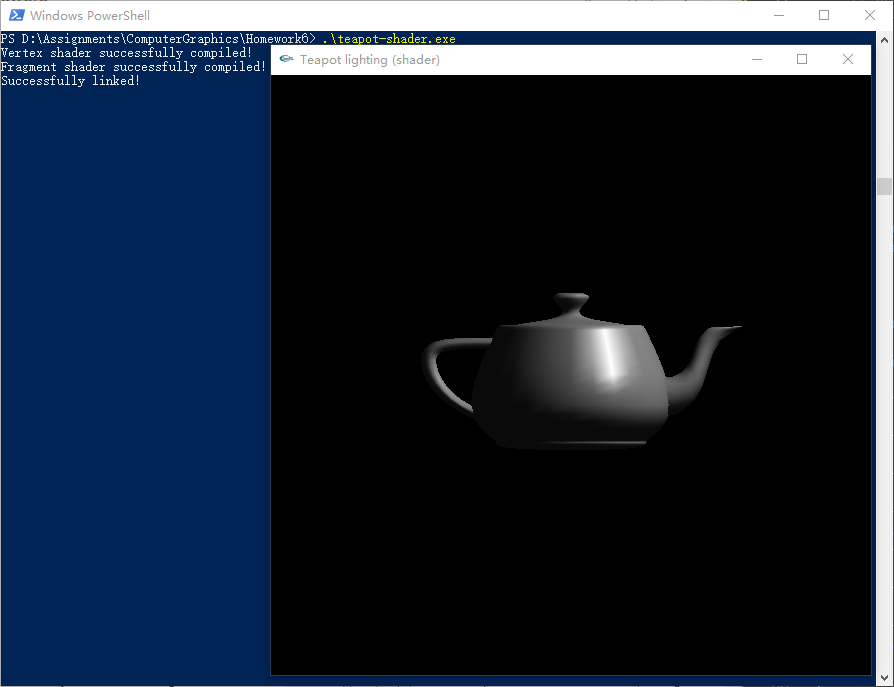
\includegraphics[width=0.9\linewidth]{fig/result-shader.png}
\caption{Teapot运行及光照结果}
\label{fig:teapot}
\end{figure}

\appendixconfig
\appendix
\section{源代码}
\subsection{固定管线(teapot.c)}
\lstinputlisting{teapot.c}

编译指令如下:
\begin{flushleft}
\verb'gcc teapot.c -lglu32 -lglut32 -lopengl32 -o teapot.exe'
\end{flushleft}

\subsection{渲染管线(teapot-shader.cpp)}
\lstinputlisting{teapot-shader.cpp}
\lstinputlisting{shader.frag}
\lstinputlisting{shader.vert}

编译指令如下:
\begin{flushleft}
\verb'g++ -Iinclude teapot-shader.c -lopengl32 -lglew32 -lglut32 -o teapot-shader.exe'
\end{flushleft}

\end{document}
% 题目: 用 OpenGL 实现简单的光照效果。
% 功能要求:
% 1. 显示默认的 Teapot 模型
% 2. 为 Teapot 模型建立 Smooth Shading 效果,如图 1 所示。
% 实现提示:
% 1. 利用 OpenGL 的 API 初始化 material property, light source, lighting model, depth buffer 等信息。
% 2. 使用 OpenGL Shader 实现。
% 3. 显示如下类似效果:

% 要求:
% 1. 作业按百分制评分, 没交作业算 0 分;
% 2. 提交代码文件,缺源代码文件的作业成绩减 10 分;
% 3. 提交直接可执行的程序文件或脚本文件,不能运行的程序(含出错,缺 dll 文件等) 作业成绩减 10 分;
% 4. 作业文档,包含简要的程序文件说明,运行方法,以及程序运行结果截图,缺文档的作业成绩减 10 分;
% 5. 发现作业抄袭的本次作业算 0 分。

% OpenGL(七) 光照模型及设置 https://blog.csdn.net/dcrmg/article/details/53121938
% http://what-when-how.com/opengl-programming-guide/creating-light-sources-opengl-programming/